\section{Part 1}

\subsection{Introduction}
I was assigned the URL \textit{www.blakersparebank.no} to perform passive reconnaissance on. I began outlining a plan of what I could do without performing any active scans, and came up with the following strategy:

\begin{enumerate}
	\item Manually crawl website to find information about employees and positions
	\item Gather information about each employee into a Maltego graph
	\item Check social network presence of employees
	\item Identify technologies used by the server hosting the website
	\item Look up nameservers \& whois-information
	\item Check if other sites are hosted on the same server - a house has many doors
\end{enumerate}

For documentation, I used \textit{CherryTree}, a fantastic text editor supporting tree-style notes (see below) and Maltego / Maltego CaseFile. I began with Maltego, but as the graph became more and more about employees, I imported the graph into Maltego CaseFile.

% CherryTree screenshot
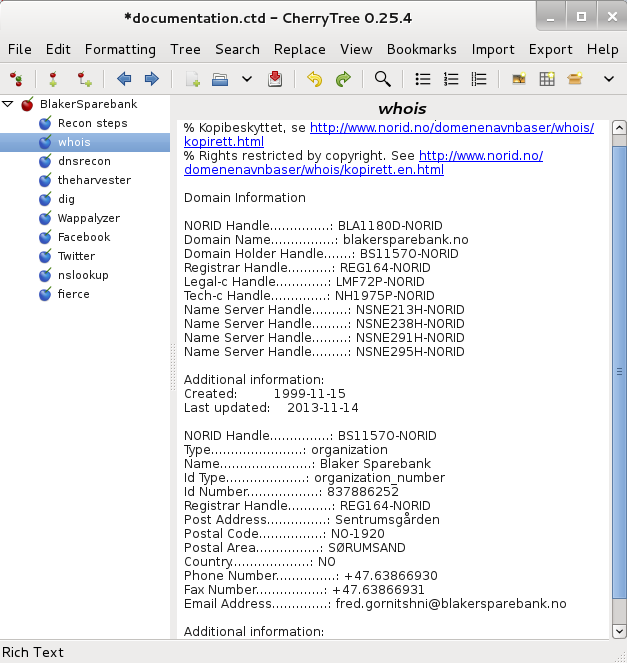
\includegraphics[scale=0.7]{cherrytree.png}\\

\subsection{Reconnaissance}
I began scanning for interesting documents (PDFs, XLS, DOC, DOCX, etc) using Google d0rks with \textit{inurl} and/or \textit{format} keys, but with no luck - or rather, with a few reports on revenue but no information I found interesting. However, the website did have an \textit{About us} section, which provided plenty of information about employees and their position. Using this, I created a plausible hierarchy of the employees (as I interpreted their positions).

I could then proceed to assign node pictures, and fetched the employee images with a short line of bash:

\begin{lstlisting}[language=bash,caption={Fetching images}]
~:# for img in $(wget -qO- http://blakersparebank.no/om-oss | \
 grep -oP '\w*\.(JPG|jpg)'); \
 do wget http://blakersparebank.no/~/media/banker/blakersparebank/ansatte/$img \
 -o Pictures/$img; done

\end{lstlisting}

Initially, I was tempted to attempt bruteforcing directories to get a better idea of the filesystem, since the image URLs gave a hint of the directory structure, but refrained from this as I presumed this fell under the category of scanning.

Setting up the Maltego graph took some time, as researching each employee is rather time consuming, but after I was done with this, I proceeded with the next step in the strategy I had outlined -- check what technologies the server used. I used \textit{Wappalyzer}, a Firefox (or, in this case, Iceweasel) addon that analyzes what technologies are used on websites by using a bunch of regex scans for signature code in HTML (meta tags/classes/scripts), URLs, response headers and global JavaScript variables, which gives a hint to what technologies may be in use.

Wappalyzer suggested BlakerSparebank was using \textit{Microsoft IIS} as a webserver, the site building on ASP.NET code. This suggests (and so did Wappalyzer) that the server is therefore running Windows Server.

This was the information I could gather from Wappalyzer:

\begin{table}[h]
\begin{tabular}{|l|l|}
\hline
OS                        & Windows Server \\ \hline
Web Server                & Microsoft IIS  \\ \hline
Language                  & ASP.NET        \\ \hline
\multirow{5}{*}{Scripts:} & jQuery         \\ \cline{2-2} 
                          & Modernizr      \\ \cline{2-2} 
                          & New Relic      \\ \cline{2-2} 
                          & yepnope.js     \\ \cline{2-2} \hline
\end{tabular}
\end{table}

Having fed this information into my graph and CherryTree, I proceeded to look up nameservers using the regular \textit{dig} command.\\

\hspace*{-5in}\begin{lstlisting}[language=bash,caption={dig'ing through DNS}]
root@battlestation:~# dig blakersparebank.no

; <<>> DiG 9.8.4-rpz2+rl005.12-P1 <<>> blakersparebank.no
;; global options: +cmd
;; Got answer:
;; ->>HEADER<<- opcode: QUERY, status: NOERROR, id: 15445
;; flags: qr rd ra; QUERY: 1, ANSWER: 1, AUTHORITY: 0, ADDITIONAL: 0

;; QUESTION SECTION:
;blakersparebank.no.		IN	A

;; ANSWER SECTION:
blakersparebank.no.	60	IN	A	153.110.253.25

;; Query time: 372 msec
;; SERVER: 192.168.0.10#53(192.168.0.10)
;; WHEN: Fri Oct 10 00:27:42 2014
;; MSG SIZE  rcvd: 52

\end{lstlisting}

This disappointed me greatly, as I had hoped for much more information, but nevertheless using the A-record for the IP I could proceed to perform a reverse DNS. Having first tried this with \textit{fierce} with no luck, I gave \textit{theharvester} a try. 

theharvester is a fantastic little program that now comes bundled with Kali as well, and harvests information from all kinds of sources. It searches Google, Bing, PGP, LinkedIn, People123, Jigsaw, as well as allows for reverse DNS lookup of a domain. It even has support for Shodan. I let it perform a full harvest on all search engines, and a reverse DNS lookup.\\

\hspace*{-5in}\begin{lstlisting}[language=bash,caption={theharvester performing full harvest}]
root@battlestation:~# theharvester -d blakersparebank.no -nhvb all

...

Full harvest..
[-] Searching in Google..
	Searching 0 results...
	Searching 100 results...
[-] Searching in PGP Key server..
[-] Searching in Bing..
	Searching 50 results...
	Searching 100 results...
[-] Searching in Exalead..

Searching 150 results...

[+] Emails found:
------------------
post@blakersparebank.no
reidun.skomdal@blakersparebank.no
blaker.sparebank@blakersparebank.no
jho@blakersparebank.no

[+] Hosts found in search engines:
------------------------------------
153.110.253.25:www.blakersparebank.no

[+] Starting active queries:
Hosts found after reverse lookup:
---------------------------------
[+] Virtual hosts:
==================
153.110.253.25	eika
153.110.253.25	surnadal-sparebank
153.110.253.25	terra-eiendomsmegling.no
153.110.253.25	tos.no
153.110.253.25	eikabk.no
153.110.253.25	aktiv.no
153.110.253.25	aurskog-sparebank.no
153.110.253.25	twocards.no
153.110.253.25	rorosbanken.no
153.110.253.25	honefossbank.no

...

[+] Shodan Database search:
153.110.253.25:www.blakersparebank.no
	Searching for: 153.110.253.25:www.blakersparebank.no
153.110.253.25:terra-eiendomsmegling.no
153.110.253.25:tos.no
153.110.253.25:eikabk.no
153.110.253.25:aktiv.no
153.110.253.25:aurskog-sparebank.no
153.110.253.25:twocards.no
153.110.253.25:rorosbanken.no
153.110.253.25:honefossbank.no

...

[+] Shodan results:
===================
\end{lstlisting}

In the output above, I cut off more than half the rows as to not make this report exceed the page limit and be able to continue with it. Although \textit{theharvester} found nothing on Shodan, and only 4 emails, it did find a plethora of domains hosted on the same server!

I began visiting these domains manually to see what they were, as the majority of them seemed to be other banks. They were indeed other banks, with nearly identical websites.

From this, and the previous information collected via Wappalyzer, I could make a qualified guess that these websites are built, run and operated with \textit{Microsoft SharePoint}.

\subsection{Summary}
The amount of information people share publicly on Facebook never cease to amaze me, and although many employees couldn't be found on Facebook, many could and several of them publicly listed their family members, work, photos, etc. I included most of this information in the Maltego graph, together with addresses, phone numbers, profiles and other information I could locate.

As for the server, I could conclude (fairly accurately I think) that it builds on ASP.NET and Microsoft SharePoint, running on a Microsoft IIS web server on a Windows Server along with plenty of other banks as virtual hosts. The downside of this is that if one of these gets compromised, they all do, as updates are often pushed simultaneously. On the other hand if one of them gets fixed, they all do as well. 

\subsubsection{Tools used}

Most of the tools I used were found in Kali under the \textit{Information Gathering} section's \textit{OSINT} or \textit{DNS} subsections, or tools I knew of previously such as \textit{Wappalyzer} or \textit{V3n0md0rk3r}.

Finally, these were the tools I used:

\begin{enumerate}
	\item \sout{Archive.org} - Trying to find useful old (cached) dox (no success)
	\item CaseFile - Another version of Maltego, more people oriented
	\item CherryTree - A treestyled notepad
	\item dig		- DNS record lookup
	\item \sout{dnsrecon} 	- For reverse DNS, but got no useful information from this tool
	\item Facebook Graph Search - Finding 3 employee Facebook profiles with \textit{People who work at BlakerSparebank}
	\item \sout{fierce}	- Also for reverse DNS, returned similar data to dnsrecon and led me nowhere.
	\item ip2location - Helped me determine that this server was operated by Evry
	\item Maltego 	- Keeping data structured in a graph
	\item \sout{Pipl.com} - Attempting to find information about employees based on name
	\item theharvester - Gathers information via a set of search engines + reverse DNS lookup
	\item Wappalyzer - Identifying server information from regex'ing returned data
	\item whois		- Query registrar for information about domain ownership
	\item \sout{V3n0md0rk3r} - Fork of smartd0rk3r for querying search engines with over 10000 Google d0rks for a specific domain to locate potential SQL-injections. Nothing found (IIS URL rewrite module activated on server)
\end{enumerate}